\section{Обзор литературы}

Перед тем, как приступить к реализации собственного драйвера USB устройства,
необходимо разобраться в том, что же такое USB,
драйверы, как они работают, как ядро Linux взаимодействует с устройствами
и какие инструменты предоставляет сама система для разработки драйверов устройств.

\subsection{Интерфейс USB}

\emph{USB (Universal Serial Bus)} -- это последовательный интерфейс, используемый для подключения
периферийных устройств к вычислительному устройству. На сегодняшний день является
основным интерфейсом подключения различной периферии к бытовой цифровой технике.

С технической точки зрения наиболее отличительной особенностью интерфейса 
является одновременная возможность передачи данных на высокой скорости
и обеспечение питания подключенной периферии.

Название Universal Serial Bus, или универсальная последовательная шина,
означает, что устройства, физически подключенные в виде древовидной структуре,
воспронимаются на логическом уровне как элементы единой шины данных, обладающей единственным
хост-контроллером, управляющим передачей информации между собой и устройствами.

Технология USB поддерживает <<горячее>> (plug'n'play) соединение устройства
с динамически загружаемыми и выгружаемыми драйверами, что позволяет пользоваться
устройством сразу после его подключения без необходимости самостоятельного запуска компонентов
операционной системы или перезагрузки хост-устройства.

Спецификация интерфейса охватывает широкий круг вопросов,
связанных с подключением и взаимодействием
периферийных устройств с вычислительной системой:
\begin{itemize}
    \item стандартизация разъемов и кабелей;
    \item нормирование электропотребления устройств;
    \item протоколы обмена данными;
    \item стандартизация функциональности и драйверов устройств.
\end{itemize}

Подробные технические сведения, а также информацию об USB, описанную
в последующих разделах, можно найти на страницах спецификации интерфейса \cite{usb}.

\subsubsection{Протоколы USB}

В отличие от RS-232 и схожих с ним последовательных интерфейсов, где формат
передаваемых данных не задан, стек интерфейса состоит из нескольких слоев протоколов,
однако, большинство контроллеров USB самостоятельно поддерживают нижние уровни стека протоколов,
поэтому они остаются незаметными для конечного разработчика.

Как уже было сказано в разделе выше, USB является последовательной шиной,
которым управляет хост, начинающий все транзакции передачи данных.

Каждая транзакция состоит из следующих частей:
\begin{itemize}
    \item Token Packet -- определяет, что передается далее;
    \item Data Packet -- необязательная, содержит полезную нагрузку;
    \item Status Packet -- возвращает статус транзакции.
\end{itemize}

Сообщение производится между хостом и определенной оконечной 
точкой устройства, называемой endpoint.

\subsubsection{Типы пакетов}

Спецификация определяет четыре различных типа пакета:
\begin{itemize}
    \item Token - определяют тип последующей транзакции;
    \item Data - содержат полезную нагрузку;
    \item Handshake - подтверждают данные или ошибки;
    \item Start Of Frame - для указания начала фрейма.
\end{itemize}

Каждый из этих типов пакетов подразделяется на собственные подтипы,
однако для нас интересны лишь подтипы, определяющие тип последующей транзакции:
\begin{itemize}
    \item In - хост хочет прочитать информацию;
    \item Out - хост хочет отправить информацию;
    \item Setup - используется для указания начала управляющих передач.
\end{itemize}

\subsubsection{Конечные точки}

Конечные точки, или endpoints, -- источники или приемники данных, относящиеся
к тому или иному устройству.

Так как шина является хост-ориентированной, конечные точки всегда находятся
на конце канала связи, поэтому сообщение с ней всегда проходит
в одностороннем порядке.

Приведем пример сообщения между хостом и конечной точкой. Предположим, что хост
отправляет некоторые данные на конечную точку. Данные приходят, после чего
помещаются в выходной буфер. Когда аппаратное обеспечение будет готово,
оно прочитает эти данные и обработает в соответствии со своей функцией.
Если же устройство хочет вернуть данные, оно помещает их во входной буфер.
Эти данные находятся там до тех пор, пока хост не отправит пакет IN, которым
он запрашивает данные этой конечной точки.

\subsubsection{Потоки сообщения}

Для описания передачи данных со стороны клиента спецификация вводит
понятие каналов (потоков) передачи данных.

\emph{Поток} -- это логическое соединение между
хостом и конечной точкой, выполняющее передачу данных.

Потоки имеют набор параметров: тип передачи,
направление потока данных, а также максимальные размеры пакета и буфера.

Простейшим примером потока является \emph{поток по умолчанию}, являющийся
двунаправленным потоком, составленным 
из нулевой входной и выходной точки с типом передачи control.

Спецификация определяет два типа потоков:
\begin{itemize}
    \item Stream Pipes -- не имеют предопределенного формата,
          являются последовательными и имеют предопределенное направление (in или out);
          поддерживают тип передачи bulk, isochronous и interrupt;

    \item Message Pipes -- имеют предопределенный формат, пересылают
          данные в нужном направлении, указанном в запросе, и таким образом
          позволяют передавать данные в двух направлениях; 
          поддерживают только тип передачи control. 
\end{itemize}

\subsubsection{Типы конечных точек}

Спецификация определяет следующие четыре типа различных конечных точек:
\begin{itemize}
    \item Control Endpoint -- используются для передач контроля;
    \item Interrupt Endpoint -- используются для передач прерываний;
    \item Isochronous Endpoint -- используются для изохронных передач;
    \item Bulk Endpoint -- используются для больших передач;
\end{itemize}

Передачи Control используются для отправки команд и операций. 
Именно эти передачи для основной настройки устройства USB 
перед началом его обслуживания хостом.

Передачи Interrupt используются в ситуациях, где требуется поведение,
аналогичное прерыванию процессора от устройства.
Поскольку все запросы исходят со стороны хоста, данные передачи
работают на механизмах опроса: устройство ставит запрос на <<прерывание>>
в очередь, пока хост не опросит устройство с целью получения этих данных.

Передачи Isochronous происходят переодически и продолжительное время. 
Обычно они содержат информацию, чувствительную к времени доставки, 
например аудио- или видеопотоки. 
Гарантируют определение ошибок с помощью контрольных сумм, 
но не гарантируют доставку, 
поскольку задержки и повторные передачи искажают изохронные данные
сильнее, чем потеря их части.

Передачи Bulk используются для передачи больших объемов данных на высокой скорости
\footnote{%
    Последний стандарт интерфейса определяет шесть спецификаций скорости передачи данных:
    USB 1.0/Low-Speed (1.5 Mbps), 
    USB 1.1/Full-Speed (14 Mbps),
    USB 2.0/Hi-Speed (480 Mbps), 
    USB 3.0/SuperSpeed (5 Gbps),
    USB 3.1/SuperSpeed\texttt{+} (10 Gbps),
    USB 3.2/SuperSpeed\texttt{++} (20 Gbps).
}.
Если полезная нагрузка меньше максимального размера пакета, то нулями она не дополняется.

\subsection{Дескрипторы USB}

Каждое USB устройство имеет сложную иерархию дескрипторов, которые описывают
некоторую информацию для хоста. К данной информации относится название устройства,
его производитель, какими способами его можно
сконфигурировать, число конечных точек, их типы и др.

Существуют следующие типы дескрипторов:
\begin{itemize}
    \item Дескрипторы устройства -- описывают сведения, относящиемся
          к общим сведениям об устройстве;  
    \item Дескрипторы конфигурации -- описывают сведения об определенной 
          конфигурации устройства;
    \item Дескрипторы интерфейса -- описывают сведения об определенном
          интерфейсе устройства;
    \item Дескрипторы конечной точки -- описывают сведения об определенной
          конечной точке устройства;
    \item Строковые декскрипторы -- содержат строковые данные.
\end{itemize}

Все перечисленные дескрипторы, за исключением строковых, ссылаются на другие
дескрипторы, в результате чего образуется дерево дескрипторов устройства,
пример которого изображен на рисунке \ref{descriptors}.

\begin{figure}[H]
    \centering
    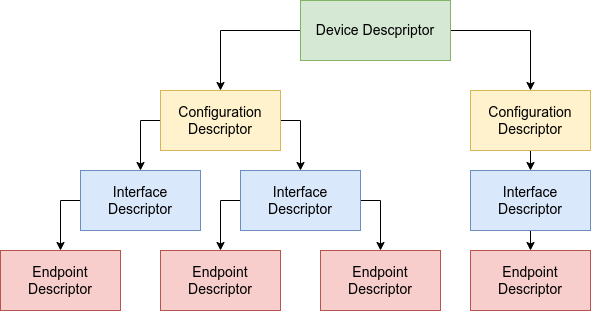
\includegraphics[scale=0.7]{Descriptors.png}
    \caption{Дескрипторы устройства USB}
    \label{descriptors}
\end{figure}

Дескриптор устройства представлен в единственном числе и включает в себя
такую информацию, как ProductID, VendorID, а также количество возможных конфигураций.

Дескриптор конфигурации указывает величину мощности, потребляемой
от последовательной шины, питается ли устройство от собственного источника,
а также количество интерфейсов, которые есть в данной конфигурации. 
Решение о выборе конфигурации принимается хостом после прочтения всех конфигураций.
%
Например, несколько конфигураций можно использовать для определения
типа питания портативного устройства: одна конфигурация будет устанавливать
высокое энергопотребление от шины, другая -- питание от аккумулятора устройства.

Дескриптор интерфейса можно рассматривать как группу конечных точек, 
выполняющую отдельную функцию устройства.

Отличительной особенностью дескриптора интерфейса является наличие у него
двух индексных полей -- bInterfaceNumber, означающий номер интерфейса,
и bAlternateSetting, которое позволяет интерфейсу выбрать альтернативную настройку.
%
По умолчанию устройство будет использовать интерфейс с наименьшим bAlternateSetting,
но хост может изменить это, отправив запрос SetInterface 
на этот интерфейс с другой bAlternateSetting.

Дескриптор конечной точки используется для указания типа точки,
ее направления, интервала опроса и максимального размера пакета.
Существует \emph{нулевая конечная точка}, 
которая используется с упомянутым ранее потоком передачи по умолчанию,
а потому не имеет дескриптора.

В данном разделе отсутствует описание полной структуры дескрипторов,
а также их полей, так как типовое взаимодействие с данными из них возложено
на инструменты, предоставляемые операционной системой.

\subsection{Класс устройств USB HID}

\emph{USB HID (Human Interface Device)} -- класс устройств,
предназначенных для взаидойствия с человеком:
клавиатура, мышь, джойстик и др.

Существует документ, описывающий дескрипторы устройств,
в частности, списки кодов функций устройств данного класса \cite{hid}.

Поскольку класс содержит множество предопределенных функций для 
каждого типа устройств, это позволяет ожидать, что устройство,
разработанное согласно спецификации класса, будет работать с программным
обеспечением, которое эту спецификацию поддерживает.

Устройства данного класса основываются на двух протоколах: 
\begin{itemize}
    \item Report protocol (протокол отчета);
    \item Boot protocol (загрузочный протокол).
\end{itemize}

Протокол отчета основан на отправке запросов и последующих отчетов со стороны устройства
об изменении статуса, например, о нажатии клавиши или движении контроллера.
Запрос со стороны хоста может содержать команду, направленную на
изменение статуса устройства, например, установка диодов на клавиатуре.

Загрузочный протокол является более простым и определен для мыши и клавиатуры.

Для предотвращения сложностей в простых взаимодействиях,
таких как в BIOS, загрузчиках операционных систем, а также драйверах одиночных клавиш, 
стандарт USB HID указывает, что клавиатуры и мыши 
могут объявлять себя <<загрузочными>> (boot-capable).
Это значит, что такие клавиатуры и мыши могут быть
переключены на более простой Boot protocol.

Переключение протокола можно осуществить с помощью специального запроса SetProtocol,
который поддерживается только <<загрузочными>> устройствами \cite{hid}.

\subsection{Обработка нажатий клавиатуры}

Так как подавляющее большинство HID устройств является boot-capable, во избежание чрезмерного
усложнения задачи, в рамках данной работы будет рассмотрена 
реализация драйвера для USB HID Boot Protocol клавиатуры.

Клавиатуры, работающие на Boot Protocol, возвращают отчет о состоянии нажатия клавиш
в упрощенном формате.

Для получения отчета достаточно отправлять запрос на входную точку клавиатуры посредством
передачи прерывания.

Размер отчета, получаемого в ответ на запрос, составляет восемь байт, хотя некоторые клавиатуры
могут предоставлять отчет меньшей длины, указанный в поле максимального размера пакета опрашиваемой
конечной точки.

\begin{table}[H] 
    \caption{Структура отчета клавиатуры}
    \begin{tabular}{| m{2cm} | m{2cm} | m{8cm} |}
        \hline
        Позиция &  Тип   & Описание                    \\
        \hline
        0       &  Байт  & Статус клавиш-модификаторов \\
        \hline
        1       &  Байт  & Зарезервирован              \\
        \hline
        2       &  Байт  & Нажатие 1                   \\
        \hline
        3       &  Байт  & Нажатие 2                   \\
        \hline
        4       &  Байт  & Нажатие 3                   \\
        \hline
        5       &  Байт  & Нажатие 4                   \\
        \hline
        6       &  Байт  & Нажатие 5                   \\
        \hline
        7       &  Байт  & Нажатие 6                   \\
        \hline
    \end{tabular}
    \label{report}
\end{table}

Из таблицы \ref{report} видно, что структура представляет собой набор байт, 
где первый байт указывает статус клавиш-модификаторов,
второй байт зарезервирован и может использоваться устройством для реализации собственной функциональности,
а оставшиеся байты представляют собой очередь нажатых клавиш.

В ряде случаев, при использовании USB клавиатуры можно достичь состояния, называемое <<фантомным состоянием>>.
Данное состояние достигается при одновременном нажатии клавиш в количестве, превышающем размер очереди нажатий
в отчете клавиатуры. В таком случае буфер нажатий клавиатуры переполняется, в отчет помещается сканкод 0x1,
и драйвер клавиатуры не вопроизводит ни одной клавиши.

Как можно заметить из таблицы \ref{report}, в отличие от регулярных клавиш, статус нажатия клавиш-модификаторов
представлен отдельным байтом, представление которого отражено в таблице \ref{modkeys}.
Данный факт можно объяснить тем, что клавиши-модификаторы как правило используются для \emph{модификации}
нажатий, и могут длительное время находится в активном состоянии.

\begin{table}[H] 
    \caption{Структура битового поля клавиш-модификаторов}
    \begin{tabular}{| m{2cm} | m{8cm} |}
        \hline
        Бит     &  Описание     \\
        \hline
        0       &  Левый Ctrl   \\
        \hline
        1       &  Левый Shift  \\
        \hline
        2       &  Левый Alt    \\
        \hline
        3       &  Левый Super  \\
        \hline
        4       &  Правый Ctrl  \\
        \hline
        5       &  Правый Shift \\
        \hline
        6       &  Правый Alt   \\
        \hline
        7       &  Правый Super \\
        \hline
    \end{tabular}
    \label{modkeys}
\end{table}

По предыдущим таблицам несложно заметить, что отчет содержит в себе лишь события, означающие
нажатие клавиш. Для того, чтобы зарегистрировать их отпускание, драйвер должен хранить предыдущий
отчет и посредством сравнения очередей определить, какая клавиша перестала быть зажатой.

\subsection{Управление светодиодами клавиатуры}

Помимо регистрации нажатий клавиш и передачи их подсистеме ввода операционной системы,
любой полноценный драйвер клавиатуры должен уметь регистрировать изменение светодиодов,
привязанных к состоянию нажатия различных клавиш фиксации.

Если в аппаратном обеспечении клавиатуры определена поддержка дополнительной выходной конечной точки,
состояние LED клавиатуры может быть установлено посредством передачи прерывания с полезной нагрузкой
размером в один байт, определяющий состояние светодиодов клавиатуры.

Однако чаще всего такая конечная точка отсутствует, и для изменения состояния светодоидов необходимо
использовать запрос SetReport используя стандартную транзакцию Setup с однобайтовым каскадом данных.
Тип Setup-запроса пакета должен быть равен 0x21, код запроса -- 0x09. Младший байт wValue запроса
должен равняться нулю, а старший байт -- значению 0x02 для индикации направления запроса \cite{osdev}.

В таблице \ref{leds} представлена структура байта, 
передаваемого для установки значения светодиодов клавиатуры.

\begin{table}[H] 
    \caption{Структура битового поля светодиодов клавиатуры}
    \begin{tabular}{| m{2cm} | m{8cm} |}
        \hline
        Бит     &  Описание                    \\
        \hline
        0       &  Num Lock                    \\
        \hline
        1       &  Caps Lock                   \\
        \hline
        2       &  Scroll Lock                 \\
        \hline
        3       &  Compose                     \\
        \hline
        4       &  Kana                        \\
        \hline
        5 - 7   &  Зарезервированы, равны нулю \\
        \hline
    \end{tabular}
    \label{leds}
\end{table}

Если значение бита соответствующего светодиода установлено в единицу, 
лампочка будет переведена в активное состояние.

Так как многие стандартные USB клавиатуры не имеют специальной выходной конечной точки для изменения
состояния LED клавиатуры, реализуемый драйвер будет поддерживать лишь клавиатуры
с интерфейсом, содержащим единственную входную конечную точку, и использовать Setup-транзакцию
для изменения состояния светодиодов.

\subsection{Драйвер клавиатуры}

В предыдущих разделах неоднократно упоминалось слово <<драйвер>>. 
Несмотря на распространенность данного термина, а также общее определение,
данное во введении, следует уточнить, что подразумевается под этим термином в данной работе.

Под \emph{драйвером устройства} понимается отдельно загружаемый компонент ядра,
называемый \emph{модулем} \footnote{%
В экосистеме Linux под модулем ядра понимают как независимо загружаемую подсистему ядра, так и всякий драйвер устройства,
работающий в пространстве ядра.
}, предоставляющий операционной системе доступ к аппаратному обеспечению данного устройства.

Важно заметить, что под драйвером ядра понимается именно компонент ядра, т.е. системный код,
исполняемый в пространстве ядра, так как существуют так называемые драйверы-фильтры, которые могут 
работать с устройством из пользовательского пространства, используя для этого функционал аппаратного драйвера.

При разработке модуля ядра необходимы знания об устройстве операционной системы, под которую разрабатывается этот модуль,
а также общие принципы и механизмы, используемые во всех операционных системах.

В рамках теоретических сведений будут описаны только те подсистемы Linux, которые необходимы для реализации функционала
устройства клавиатуры.

Сведения, относящиеся к общим положениям организации аппаратного обеспечения и операционных систем будут либо упомянуты
в разделах, непосредственно связанных с описанием реализации драйвера, 
либо опущены как не требующие подробного представления для понимания принципов работы кода.

Подробное изложение всех теоретических сведений, 
используемых при разработке модулей USB устройств, может быть найдено как в определенных
разделах документации ядра Linux, поддерживаемой сообществом, так и в соответствующей узкоспециализированной литературе,
посвященной данной тематике \cite{ldd3}.

\subsection{Подсистема USB Linux}

\emph{USB Core} -- это подсистема ядра Linux, созданная для поддержки USB-устройств и контроллеров USB-шины. 
Данная подсистема определяет набор структур, макросов и функций, позволяя разработчикам системного кода абстрагироваться
от аппаратной реализации USB и относящихся к ней аппаратно-зависимых функций.

Помимо реализации через различные компоненты ядра таких механизмов как <<горячее подключение>> устройств с последующим
запуском подходящего модуля, подсистема предоставляет разработчикам единообразный программный интерфейс для разработки
переносимых драйверов устройств.

Определение группы устройств, которую может обслуживать драйвер, а также функций, используемых в качестве обработчиков
стандартных событий (например, подключение и отключение устройства), осуществляются через определение специальной
структуры.

Сообщение между хостом и устройством осуществляется при помощи \emph{URB (USB Request Block)}, блоков запросов,
регистрируемых в подсистеме с возможностью повторного использования.

Многие аппаратно-зависимые функции, начиная с настройки устройства, заканчивая созданием когерентной памяти 
для совместного доступа со стороны процессора и устройства, также реализованы в виде специальных функций \cite{usbapi}.

\subsection{Подсистема ввода Linux}

В то время как подсистема универсальной последовательной шины предоставляет возможность взаимодействия между драйвером и устройством,
подсистема ввода Linux позволяет драйверу устройства ввода реализовать передачу сведений в пользовательское пространство
в виде манипуляций ввода.

На рисунке \ref{input-core} изображена диаграмма взаимодействия подсистемы ввода Linux с другими модулями ядра.

\begin{figure}[H]
    \centering
    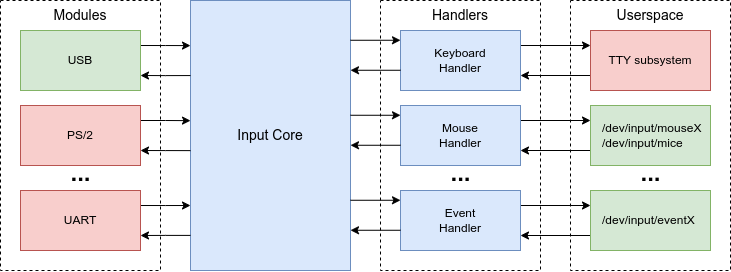
\includegraphics[scale=0.625]{Input_Subsystem.png}
    \caption{Подсистема ввода Linux}
    \label{input-core}
\end{figure}

Из представленной выше диаграммы видно, что Input Core является таким же посредником, как и подсистема USB: для того,
чтобы модуль устройства мог функционировать как устройство ввода, достаточно зарегистрировать специальную структуру, описывающую 
данное устройство ввода, и использовать функции сообщения от имени этого устройства к подсистеме ввода. 
Последующее взаимодействие с подсистемой сводится к сообщению о возникновении нового события ввода, 
работа по регистрации и обработке этих событий лежит на самой подсистеме ввода и разнообразных обработчиках событий \cite{inputsubsystem}.

Как и в случае с подсистемой универсальной последовательной шины, подсистема ввода предоставляет специальную структуру,
определяющую устройство ввода, набор функций для его регистрации, 
а также функции для сообщения подсистеме ввода новых событий ввода.

Стоит отметить, что несмотря на большое количество функционала, делигированного подсистеме ввода, модуль клавиатуры
все еще должен заниматься некоторыми преобразованиями данных, получаемых от аппаратной части устройства, 
для последующей передачи в подсистему ввода. 
Это связано с тем, что Linux и Windows на уровне ядра работают с так называемыми raw-сканкодами, в то время как
Boot Protocol клавиатуры возвращает USB-коды клавиш \cite{deskthority}.
Для преобразования кодов в <<сырые>> сканкоды может быть использована специальная таблица \cite{scancodes}.